\documentclass[conference]{IEEEtran}
\IEEEoverridecommandlockouts

\usepackage{cite}
\usepackage{amsmath,amssymb,amsfonts}
\usepackage{graphicx}
\usepackage{textcomp}
\usepackage{xcolor}
\usepackage{tikz}
\usepackage{booktabs}
\usepackage{multirow}
\usepackage{url}
\usepackage{hyperref}
\usetikzlibrary{shapes.geometric, arrows.meta, positioning, calc, fit, backgrounds}

\hypersetup{
  colorlinks=true,
  linkcolor=black,
  citecolor=black,
  urlcolor=blue,
  bookmarks=true,
  pdfauthor={Tharaka Dilshan et al.},
  pdftitle={Diffusion-Based Counterfactual ECG Generation for Atrial Fibrillation Data Augmentation}
}

\begin{document}

\title{Diffusion-Based Counterfactual ECG Generation\\for Atrial Fibrillation Data Augmentation}

\author{
\IEEEauthorblockN{Tharaka Dilshan, Nethmini Karunarathne, Isuri Devindi\textsuperscript{*}}
\IEEEauthorblockA{\textit{Dept. Computer Engineering},
\textit{University of Peradeniya}, Sri Lanka\\
\textsuperscript{*}\textit{Also with Dept. Electrical \& Computer Engineering,}\\
\textit{University of Maryland, College Park, USA}}
\and
\IEEEauthorblockN{Molly Maleckar, Vajira Thambawita}
\IEEEauthorblockA{\textit{SimulaMet}\\
Oslo, Norway}
\and
\IEEEauthorblockN{Roshan Ragel, Isuru Nawinne}
\IEEEauthorblockA{\textit{Dept. Computer Engineering}\\
\textit{University of Peradeniya}, Sri Lanka}
}

\maketitle

\begin{abstract}
\textbf{Objective:} Automated detection of atrial fibrillation (AFib) using deep learning requires large, balanced ECG datasets, yet clinical data remains scarce, imbalanced, and constrained by privacy regulations.
\textbf{Methods:} We present a diffusion-based data augmentation pipeline that generates synthetic ECG segments by transforming existing recordings into counterfactual waveforms of the opposing class. The pipeline employs an SDEdit-style \cite{meng2022sdedit} conditional denoising process with classifier-free guidance, operating on single-lead ECG signals from the MIMIC-IV ECG database. A content-style disentangled UNet architecture separates class-invariant morphology from class-discriminative rhythm features. A multi-stage plausibility validator enforces morphological, physiological, and clinical constraints, retaining only waveforms that satisfy quality thresholds.
\textbf{Results:} We evaluate the augmented data through a three-regime protocol using a ResNet-BiLSTM classifier: training on originals only (A), on counterfactuals only (B), and on an augmented mixture with 33.33\% counterfactuals (C). The augmented condition achieves 95.05\% accuracy and 98.60\% AUROC, statistically equivalent to original-only training (95.63\% accuracy, $p_{\text{TOST}}=0.007$, $\Delta=\pm2\%$), while counterfactual-only training retains 89.9\% of original performance.
\textbf{Conclusion:} None of the accepted counterfactuals are near-copies of training data (maximum correlation to nearest original: 0.30), confirming that the pipeline produces novel, privacy-preserving synthetic signals suitable for dataset balancing.
\end{abstract}

\begin{IEEEkeywords}
atrial fibrillation, ECG augmentation, diffusion models, counterfactual generation, data balancing
\end{IEEEkeywords}

\section{Introduction}

Atrial fibrillation (AFib) is the most common sustained cardiac arrhythmia, affecting over 37 million individuals worldwide and significantly increasing the risk of stroke, heart failure, and mortality \cite{andersen2019}. Early and reliable detection from electrocardiogram (ECG) recordings is critical for timely intervention. Deep learning models have demonstrated strong AFib detection performance on curated datasets \cite{petmezas2021}, but translating these results into practical clinical tools faces two persistent barriers.

First, ECG datasets exhibit severe class imbalance. As documented in multiple studies \cite{petmezas2021, delaney2019}, normal sinus rhythm recordings vastly outnumber AFib episodes, biasing classifiers toward the majority class and reducing sensitivity to the arrhythmia of interest. Second, ECG signals carry subject-specific morphological signatures that persist even after metadata removal, introducing privacy concerns that limit cross-institutional data sharing.

Traditional augmentation techniques such as scaling, jittering, and time warping can improve model robustness but do not introduce physiologically meaningful rhythm variations. A scaled version of a normal ECG does not exhibit the hallmark features of AFib: irregular R-R intervals, absence of P-waves, and fibrillatory baseline activity. Generative models offer a principled alternative by learning the distribution of ECG signals and synthesizing new examples that capture class-specific characteristics. Counterfactual generation is particularly well-suited to this setting: each real recording can be transformed into a plausible example of the opposing class, simultaneously addressing class imbalance (by producing minority-class examples from majority-class recordings) and privacy constraints (by generating synthetic signals that share no subject-specific signatures with originals).

Among generative approaches, diffusion models have recently demonstrated superior sample quality compared to GANs \cite{goodfellow2014} and VAEs \cite{kingma2014} across image and audio domains. Their iterative denoising process avoids the mode collapse observed in GAN training \cite{delaney2019} and the blurry reconstructions characteristic of VAEs \cite{bredell2023}. The SDEdit framework \cite{meng2022sdedit} enables content-guided generation by starting from a partially corrupted version of a real signal and denoising toward a target distribution. This preserves structural properties of the source waveform while introducing class-appropriate modifications.

In this work, we adopt this diffusion-based strategy to transform existing ECG recordings into counterfactual waveforms of the opposing class. A multi-stage plausibility validator retains only waveforms that satisfy clinical constraints. We evaluate augmentation utility through a three-regime protocol and demonstrate statistical equivalence between augmented and original-only training.

\subsection{Contributions}
Our contributions are:
\begin{itemize}
  \item A content-style disentangled diffusion pipeline combining SDEdit sampling, classifier-free guidance, and multi-stage plausibility validation.
  \item A three-regime evaluation protocol with formal equivalence testing (TOST, non-inferiority) to quantify augmentation safety.
  \item Empirical evidence that filtered counterfactuals are statistically equivalent to real data for classifier training and contain zero near-copies of training examples.
\end{itemize}


\section{Related Work}

Table~\ref{tab:related} summarizes representative ECG generation approaches.

\begin{table}[t]
\centering
\caption{Comparison of ECG Generation Approaches}
\label{tab:related}
\begin{tabular}{lccc}
\toprule
\textbf{Method} & \textbf{Type} & \textbf{CF} & \textbf{Key Challenge} \\
\midrule
WGAN-GP \cite{gulrajani2017} & GAN & No & Mode collapse\textsuperscript{a} \\
CoFE-VAE \cite{nemirovsky2021} & VAE & Yes & Reconstruction quality\textsuperscript{b} \\
CoFE-GAN \cite{jang2025cofe} & GAN & Yes & Iterative inversion \\
DDPM \cite{ho2020} & Diff. & No & Sampling speed \\
\textbf{Ours} & Diff. & Yes & See Sec.~\ref{sec:limitations} \\
\bottomrule
\end{tabular}

\vspace{1mm}
\footnotesize{\textsuperscript{a}Mode collapse documented in ECG synthesis by \cite{delaney2019}.}
\footnotesize{\textsuperscript{b}VAE reconstruction limitations discussed in \cite{bredell2023}.}
\end{table}

\subsection{ECG Generation and Augmentation}
Generative adversarial networks (GANs) \cite{goodfellow2014} have been applied to ECG synthesis with varying results. As part of our preliminary work, we implemented a WGAN-GP-based \cite{gulrajani2017} counterfactual generator and observed mode collapse and latent-space artifacts during optimization, consistent with the findings of Delaney et al. \cite{delaney2019}, who reported similar instabilities in GAN-based ECG synthesis. CoFE-VAE \cite{nemirovsky2021} uses variational autoencoders for time-series counterfactuals. However, VAE-based methods are known to produce overly smooth outputs due to the averaging effect of maximum likelihood training, as analyzed in \cite{bredell2023}. CoFE-GAN \cite{jang2025cofe} combines GANs with gradient-based latent descent but relies on iterative inversion during generation, which increases computational cost. Our pipeline operates directly in waveform space and avoids separate encoder-decoder inversion steps.

\subsection{Diffusion Models for Time Series}
Denoising diffusion probabilistic models (DDPMs) \cite{ho2020} generate samples through iterative denoising from Gaussian noise. DDIM \cite{song2021ddim} accelerates sampling via deterministic updates. SDEdit \cite{meng2022sdedit} enables guided editing by initializing from partially noised data. Classifier-free guidance (CFG) \cite{ho2022classifier} steers generation toward target classes by training the model with random class label dropout, so that during inference both conditional and unconditional predictions can be combined without requiring a separately trained classifier. DiffStyleTS \cite{nagda2025diffstylts} introduces a diffusion-based framework for style transfer in time series through content-style disentanglement, demonstrating the effectiveness of separating invariant content from class-discriminative style representations. Recent extensions to medical time series \cite{alcaraz2023diffusion} demonstrate improved fidelity over GAN-based alternatives.

\subsection{Equivalence Testing in Augmentation}
Standard hypothesis testing (paired $t$-test) can detect differences but cannot establish equivalence. The Two One-Sided Tests (TOST) procedure \cite{schuirmann1987comparison} tests whether two means lie within a predefined equivalence margin $\Delta$. Non-inferiority testing \cite{walker2011understanding} establishes that a new method is no worse than a reference by more than a clinically acceptable margin. We adopt both tests applied to per-fold accuracy values to formally quantify augmentation safety.


\section{Methodology}

\subsection{Dataset and Preprocessing}

We use the MIMIC-IV ECG Diagnostic Electrocardiogram Matched Subset \cite{mimiciv_ecg}, a publicly available collection of clinical 12-lead ECG recordings. We extract Lead~II signals and classify them as Normal (sinus rhythm) or AFib based on clinical report annotations. After filtering and class-balancing, each recording is resampled to 250~Hz and cleaned using NeuroKit2 (bandpass 0.5--40~Hz). Signals are segmented into non-overlapping 10-second windows (2,500 samples). Global normalization scales all segments to $[-1.5, 1.5]$ using training-set-wide extrema, preserving relative amplitude differences and avoiding per-segment clipping artifacts. Table~\ref{tab:dataset} summarizes the processed dataset.

\begin{table}[t]
\centering
\caption{Dataset Summary After Preprocessing}
\label{tab:dataset}
\begin{tabular}{lrr}
\toprule
\textbf{Partition} & \textbf{Segments} & \textbf{Normal / AFib} \\
\midrule
Training   & 104,855 & 52,447 / 52,408 \\
Validation &  22,469 & 11,239 / 11,230 \\
Test       &  22,469 & 11,239 / 11,230 \\
\midrule
\textbf{Total} & \textbf{149,793} & \textbf{74,925 / 74,868} \\
\bottomrule
\end{tabular}
\end{table}

\subsection{AFib Classification Model}

The downstream classifier combines a multi-scale convolutional front-end (parallel 1D convolutions at kernel sizes 3, 7, and 15), a ResNet-34 backbone, a bidirectional LSTM for temporal modeling, and a self-attention module. Training uses focal loss ($\alpha{=}0.65$, $\gamma{=}2.0$), Adam optimizer (lr$=10^{-3}$), early stopping at 15 epochs patience on validation AUROC, and ReduceLROnPlateau scheduling.

\subsection{Diffusion Model Architecture}

The generative model consists of three components (Fig.~\ref{fig:architecture}):

\textbf{Content Encoder.} Inspired by the content-style disentanglement framework of DiffStyleTS \cite{nagda2025diffstylts}, we extract class-invariant morphological features. Five convolutional layers with BatchNorm and LeakyReLU map the input ECG to a 256-dimensional latent vector using the VAE reparameterization trick, capturing waveform shape independent of rhythm class.

\textbf{Style Encoder.} Extracts class-discriminative rhythm features. Four convolutional layers with InstanceNorm produce a 128-dimensional style vector. An auxiliary classification head predicts the class from the style vector during training, encouraging disentanglement.

\textbf{Conditional UNet.} A 1D UNet with channel multipliers $(1, 2, 4, 8) \times 64$, two residual blocks per level, and self-attention at the two lowest resolutions. Conditioning is injected through sinusoidal timestep embeddings (256-d), content embeddings, style embeddings, and a learned class embedding with classifier-free guidance dropout (10\%).

\textbf{Training.} The model is trained in two stages. \textit{Stage~1 (epochs 1--50, reconstruction):} All three components are trained jointly to minimize a weighted combination of MSE noise-prediction loss (weight~1.0), style-encoder classification cross-entropy (weight~0.5) that encourages the style vector to capture class-discriminative features, and a KL-divergence term (weight~0.01) that regularizes the content encoder's VAE latent space. \textit{Stage~2 (epochs 51--100, counterfactual fine-tuning):} The reconstruction loss is retained (weight~1.0) and two additional objectives are introduced: a classifier flip loss (weight~1.0) that penalizes generated counterfactuals not classified as the target class, and a similarity loss (weight~0.3) that preserves morphological fidelity via MSE between the generated signal and the original. Total training requires approximately 21.6 hours on an NVIDIA RTX 6000 Ada Generation GPU (48~GB). The model contains 19.1M parameters.

\begin{figure*}[t]
\centering
\resizebox{0.97\textwidth}{!}{%
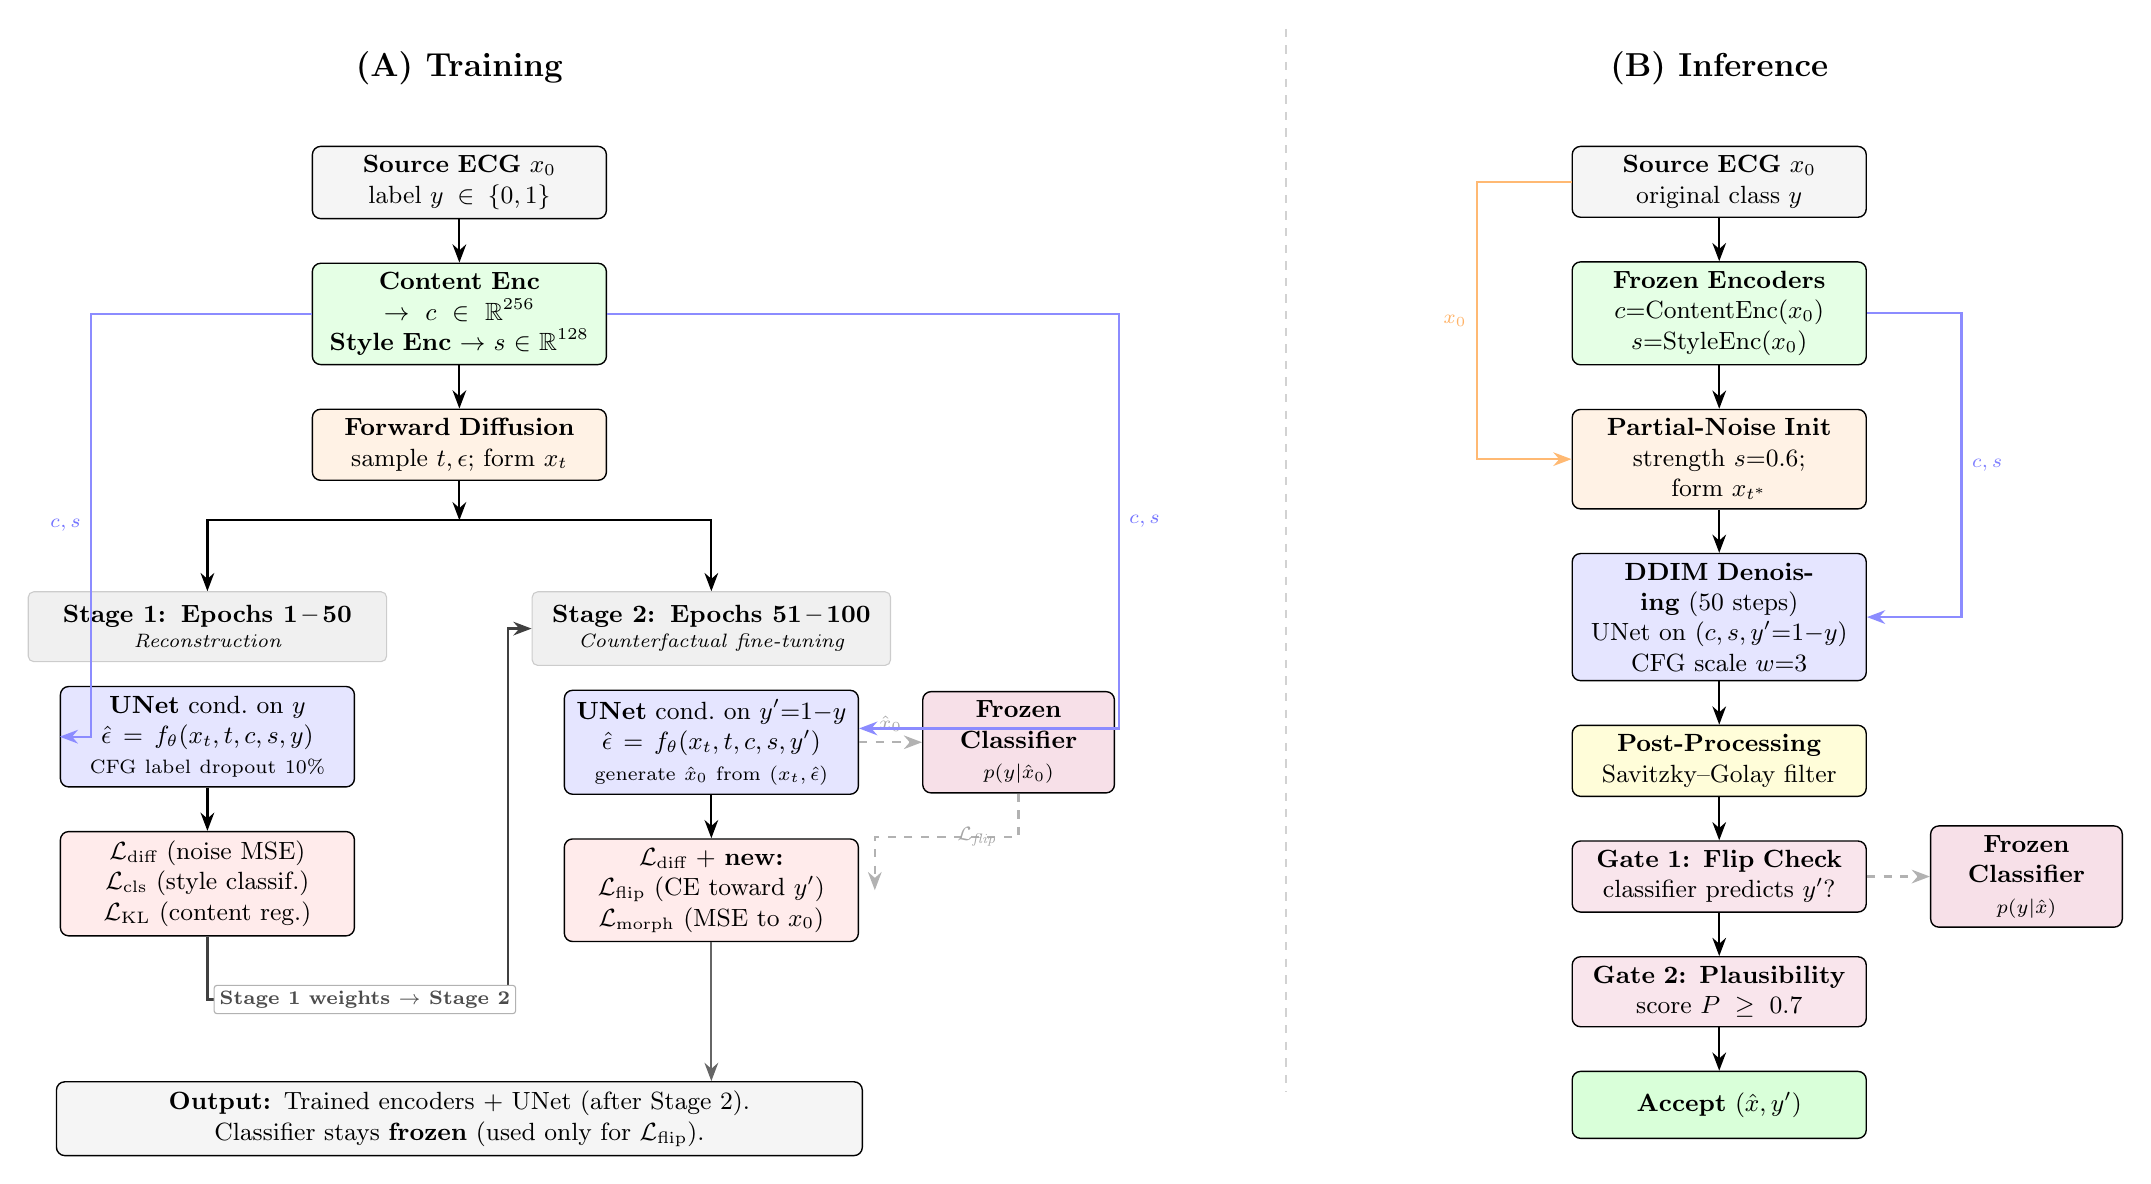
\begin{tikzpicture}[
  font=\small,
  >=Stealth,
  box/.style={rectangle, draw, rounded corners=3pt, align=center,
              minimum height=0.85cm, text width=3.5cm, fill=#1, line width=0.5pt},
  box/.default=white,
  wbox/.style={rectangle, draw, rounded corners=3pt, align=center,
              minimum height=0.85cm, text width=10.0cm, fill=#1, line width=0.5pt},
  heading/.style={font=\bfseries\large, align=center},
  stagelab/.style={font=\bfseries\small, fill=gray!12, draw=gray!40,
                   rounded corners=2pt, inner sep=5pt, text width=4.2cm, align=center},
  arr/.style={->, thick, >=Stealth},
  condarr/.style={->, line width=0.8pt, >=Stealth, color=blue!45},
  srcarr/.style={->, line width=0.8pt, >=Stealth, color=orange!55},
  darr/.style={->, thick, dashed, >=Stealth, color=gray!60},
  grayarr/.style={->, line width=0.7pt, >=Stealth, color=gray!55},
]
% --- (A) TRAINING ---
\node[heading] (title_train) at (0, 0) {(A) Training};
\node[box=gray!8, below=0.65cm of title_train] (input) {
  \textbf{Source ECG} $x_0$\\label $y \in \{0,1\}$};
\node[box=green!10, below=0.55cm of input] (encoders) {
  \textbf{Content Enc} $\to c \in \mathbb{R}^{256}$\\
  \textbf{Style Enc} $\to s \in \mathbb{R}^{128}$};
\node[box=orange!10, below=0.55cm of encoders] (fwd_diff) {
  \textbf{Forward Diffusion}\\sample $t, \epsilon$; form $x_t$};
\draw[arr] (input) -- (encoders);
\draw[arr] (encoders) -- (fwd_diff);
\coordinate (branch) at ($(fwd_diff.south) + (0,-0.5)$);
\draw[arr] (fwd_diff.south) -- (branch);
% Stage 1
\node[stagelab, below=1.4cm of fwd_diff, xshift=-3.2cm] (s1_lab) {
  Stage 1: Epochs 1\,--\,50\\[-2pt]
  {\normalfont\itshape\scriptsize Reconstruction}};
\node[box=blue!10, below=0.3cm of s1_lab] (unet_s1) {
  \textbf{UNet} cond.\ on $y$\\
  $\hat\epsilon = f_\theta(x_t, t, c, s, y)$\\
  {\scriptsize CFG label dropout 10\%}};
\node[box=red!8, below=0.55cm of unet_s1] (loss_s1) {
  $\mathcal{L}_\text{diff}$ (noise MSE)\\
  $\mathcal{L}_\text{cls}$ (style classif.)\\
  $\mathcal{L}_\text{KL}$ (content reg.)};
\draw[arr] (branch) -| (s1_lab.north);
\draw[arr] (unet_s1) -- (loss_s1);
% Stage 2
\node[stagelab, below=1.4cm of fwd_diff, xshift=3.2cm] (s2_lab) {
  Stage 2: Epochs 51\,--\,100\\[-2pt]
  {\normalfont\itshape\scriptsize Counterfactual fine-tuning}};
\node[box=blue!10, below=0.3cm of s2_lab] (unet_s2) {
  \textbf{UNet} cond.\ on $y'{=}1{-}y$\\
  $\hat\epsilon = f_\theta(x_t, t, c, s, y')$\\
  {\scriptsize generate $\hat{x}_0$ from $(x_t, \hat\epsilon)$}};
\node[box=red!8, below=0.55cm of unet_s2] (loss_s2) {
  $\mathcal{L}_\text{diff}$ + \textbf{new:}\\
  $\mathcal{L}_\text{flip}$ (CE toward $y'$)\\
  $\mathcal{L}_\text{morph}$ (MSE to $x_0$)};
\draw[arr] (branch) -| (s2_lab.north);
\draw[arr] (unet_s2) -- (loss_s2);
% Frozen classifier (Stage 2)
\node[box=purple!12, text width=2.2cm, right=0.8cm of unet_s2] (clf_s2) {
  \textbf{Frozen}\\
  \textbf{Classifier}\\
  {\scriptsize $p(y|\hat{x}_0)$}};
\draw[darr] (unet_s2.east) -- (clf_s2.west)
  node[midway, above, font=\scriptsize\itshape, text=gray!70] {$\hat{x}_0$};
\draw[darr] (clf_s2.south) -- ++(0,-0.55) -| ([xshift=0.2cm]loss_s2.east)
  node[pos=0.25, right, font=\scriptsize\itshape, text=gray!70] {$\mathcal{L}_\text{flip}$};
% Encoder conditioning arrows — routed OUTSIDE the stage boxes
% Left: go far left (x offset -2.8) to avoid overlapping Stage 1 boxes
\draw[condarr] (encoders.west) -- ++(-2.8, 0) |- (unet_s1.west)
  node[pos=0.25, left, font=\scriptsize, text=blue!55] {$c, s$};
% Right: go far right (beyond frozen classifier) to avoid overlapping Stage 2 boxes
% Enters UNet slightly above center to separate from the dashed x̂₀ arrow leaving u2.east
\draw[condarr] (encoders.east) -- ++(6.5, 0) |- ([yshift=5pt]unet_s2.east)
  node[pos=0.25, right, font=\scriptsize, text=blue!55] {$c, s$};
%
% ---- SEQUENTIAL ARROW: Stage 1 → Stage 2 ----
% From Stage 1 loss, down, then through gap between stages, up into Stage 2 label
\coordinate (seq_btm) at ($(loss_s1.south) + (0,-0.8)$);
\draw[->, thick, >=Stealth, color=black!75]
  (loss_s1.south) -- (seq_btm) -| ([xshift=-0.3cm]s2_lab.west) -- (s2_lab.west);
\node[font=\scriptsize\bfseries, text=black!70, fill=white, inner sep=2pt,
      draw=black!30, rounded corners=1pt]
  at ($(seq_btm) + (2.0, 0)$) {Stage~1 weights $\rightarrow$ Stage~2};
%
% ---- OUTPUT BOX (only from Stage 2) ----
\node[wbox=gray!8, below=1.8cm of $(loss_s1.south)!0.5!(loss_s2.south)$] (train_out) {
  \textbf{Output:} Trained encoders + UNet (after Stage~2). Classifier stays \textbf{frozen} (used only for $\mathcal{L}_\text{flip}$).};
% Arrow from Stage 2 loss straight down to output box
\draw[->, thick, >=Stealth, color=black!60]
  (loss_s2.south) -- (loss_s2.south |- train_out.north);
% --- (B) INFERENCE ---
\node[heading] (title_infer) at (16, 0) {(B) Inference};
\node[box=gray!8, below=0.65cm of title_infer] (inf_input) {
  \textbf{Source ECG} $x_0$\\original class $y$};
\node[box=green!10, below=0.55cm of inf_input] (inf_enc) {
  \textbf{Frozen Encoders}\\
  $c{=}\text{ContentEnc}(x_0)$\\
  $s{=}\text{StyleEnc}(x_0)$};
\node[box=orange!10, below=0.55cm of inf_enc] (inf_noise) {
  \textbf{Partial-Noise Init}\\
  strength $s{=}0.6$; form $x_{t^*}$};
\node[box=blue!10, below=0.55cm of inf_noise] (inf_ddim) {
  \textbf{DDIM Denoising} (50 steps)\\
  UNet on $(c, s, y'{=}1{-}y)$\\
  CFG scale $w{=}3$};
\node[box=yellow!15, below=0.55cm of inf_ddim] (inf_post) {
  \textbf{Post-Processing}\\
  Savitzky--Golay filter};
\node[box=purple!10, below=0.55cm of inf_post] (inf_gate1) {
  \textbf{Gate 1: Flip Check}\\
  classifier predicts $y'$?};
\node[box=purple!10, below=0.55cm of inf_gate1] (inf_gate2) {
  \textbf{Gate 2: Plausibility}\\
  score $P \ge 0.7$};
\node[box=green!15, below=0.55cm of inf_gate2] (inf_accept) {
  \textbf{Accept} $(\hat{x}, y')$};
\draw[arr] (inf_input) -- (inf_enc);
\draw[arr] (inf_enc) -- (inf_noise);
\draw[arr] (inf_noise) -- (inf_ddim);
\draw[arr] (inf_ddim) -- (inf_post);
\draw[arr] (inf_post) -- (inf_gate1);
\draw[arr] (inf_gate1) -- (inf_gate2);
\draw[arr] (inf_gate2) -- (inf_accept);
\draw[srcarr] (inf_input.west) -- ++(-1.2,0) |- (inf_noise.west)
  node[pos=0.25, left, font=\scriptsize, text=orange!60] {$x_0$};
\draw[condarr] (inf_enc.east) -- ++(1.2,0) |- (inf_ddim.east)
  node[pos=0.25, right, font=\scriptsize, text=blue!50] {$c, s$};
\node[box=purple!12, text width=2.2cm, right=0.8cm of inf_gate1] (inf_clf) {
  \textbf{Frozen}\\
  \textbf{Classifier}\\
  {\scriptsize $p(y|\hat{x})$}};
\draw[darr] (inf_gate1.east) -- (inf_clf.west);
% Separator — perfectly vertical at fixed x = 10.5
\draw[dashed, line width=0.8pt, gray!35] (10.5, 0.5) -- (10.5, -13.0);
\end{tikzpicture}
}
\caption{Overview of the proposed pipeline. \textbf{(A)~Training} proceeds in two stages using the same architecture: Stage~1 (epochs 1--50) trains the UNet for noise reconstruction conditioned on the original label $y$; Stage~2 (epochs 51--100) fine-tunes the same UNet for counterfactual generation by conditioning on the target label $y'{=}1{-}y$ and introducing classifier flip ($\mathcal{L}_\text{flip}$) and morphology preservation ($\mathcal{L}_\text{morph}$) losses. The classifier remains frozen throughout. \textbf{(B)~Inference:} partial-noise initialization corrupts the source ECG, DDIM denoising with classifier-free guidance generates the counterfactual toward $y'$, and two gates (flip verification + plausibility) filter the output.}
\label{fig:architecture}
\end{figure*}

\subsection{Counterfactual Generation via SDEdit}

Both the content and style encoders receive the \textit{same source ECG} as input. The content encoder extracts class-invariant morphological features (waveform shape, amplitude patterns) that should be preserved in the counterfactual. The style encoder extracts class-discriminative rhythm features (R-R regularity, P-wave characteristics) that inform the current class identity.

We initialize generation from a partially noised version of the source using the SDEdit approach \cite{meng2022sdedit}. Given source signal $x_0$ with label $y$:
\begin{equation}
x_t = \sqrt{\bar{\alpha}_t}\, x_0 + \sqrt{1 - \bar{\alpha}_t}\, \epsilon, \quad \epsilon \sim \mathcal{N}(0, I)
\end{equation}
where $t = \lfloor s \cdot T \rfloor$ and strength $s{=}0.6$ controls the corruption level. The UNet then denoises $x_t$ over 50 DDIM steps, conditioned on the content embedding (to preserve morphology), the style embedding, and the \textit{target class label} $y' = 1 - y$. Class-steering uses classifier-free guidance (CFG) with scale $w{=}3.0$:
\begin{equation}
\hat{\epsilon} = \epsilon_\theta(x_t, t, \varnothing) + w\bigl(\epsilon_\theta(x_t, t, y') - \epsilon_\theta(x_t, t, \varnothing)\bigr)
\end{equation}
The scale $w$ amplifies the difference between conditional and unconditional noise predictions: $w{=}1$ uses only the conditional prediction, while larger values strengthen adherence to the target class at the cost of sample diversity. Post-processing applies a Savitzky-Golay filter \cite{savgol} (window 11, order 3) to suppress high-frequency artifacts.

\subsection{Plausibility Validation and Filtering}

Each generated waveform is scored by a three-tier validator. The specific thresholds below are chosen based on established clinical ranges for ECG parameters \cite{clifford2006}:

\textbf{Morphology} (weight 0.3): amplitude within $\pm 3$ normalized units (signals are globally scaled to $[-1.5, 1.5]$), at least 3 R-peaks per 10~s (corresponding to $\geq$18~BPM, below which the signal is likely artifact), QRS integrity above 70\%, and fewer than 1\% outlier samples.

\textbf{Physiology} (weight 0.3): R-R intervals within 0.24--2.0~s (corresponding to 30--250~BPM, the physiologically viable heart rate range \cite{clifford2006}), and R-R coefficient of variation below 0.5.

\textbf{Clinical directionality} (weight 0.4): For Normal-to-AFib, R-R irregularity must increase by at least 30\%; for AFib-to-Normal, it must decrease by at least 20\%. These asymmetric thresholds reflect the observation that AFib inherently exhibits greater rhythm variability than normal sinus rhythm.

The weighted plausibility score $P = 0.3 M + 0.3 \Phi + 0.4 C$ must exceed 0.7. Rejected samples are regenerated up to three times. After filtering, 7,784 counterfactuals (balanced across classes) passed validation with mean plausibility $0.76 \pm 0.04$.


\section{Experimental Results}

We evaluate the proposed pipeline along two axes: first, the quality and novelty of the generated counterfactual ECGs themselves, and second, their utility as training data for downstream AFib classification.

\subsection{Counterfactual Signal Quality and Plausibility}

Table~\ref{tab:quality} summarizes generation quality metrics measured on 2,000 randomly sampled counterfactuals. The PSNR of 10.19~dB reflects intentional class-specific modifications rather than noise corruption. The near-zero mean correlation ($r{=}0.0003$) confirms that generated signals undergo substantial waveform transformation, as expected for counterfactual class conversion. Generated signals exhibit slightly higher SNR (15.7~dB vs. 14.2~dB for originals) due to the smoothing effect of the diffusion denoising process. The KS statistic of 0.092 indicates that the amplitude distributions of original and generated signals remain closely aligned (values near 0 denote identical distributions), while the Wasserstein distance of 0.008 confirms minimal distributional shift.

\begin{table}[t]
\centering
\caption{Generation Quality Metrics}
\label{tab:quality}
\begin{tabular}{lc}
\toprule
\textbf{Metric} & \textbf{Value} \\
\midrule
PSNR (source vs. CF)       & $10.19 \pm 3.81$ dB \\
SNR (original / generated)  & 14.24 / 15.74 dB \\
Correlation (source vs. CF) & $0.0003 \pm 0.068$ \\
Plausibility score           & $0.76 \pm 0.04$ \\
Plausibility $\geq 0.7$     & 100\% (of accepted CFs) \\
KS statistic (amplitude)    & 0.092 \\
Wasserstein distance         & 0.008 \\
\bottomrule
\end{tabular}
\end{table}

\subsection{Uniqueness and Privacy Verification}

To rule out memorization, we compute the maximum Pearson correlation between each of 500 sampled counterfactuals and 2,000 same-class training originals. The mean maximum correlation is $0.30 \pm 0.07$, well below the threshold of 0.80 commonly used to flag near-duplicate signals in ECG databases \cite{clifford2006}. The mean L2 distance to the nearest training example is $0.058 \pm 0.033$ on z-normalized signals. No sample exceeds 0.80 correlation, confirming that the pipeline generates genuinely novel waveforms rather than retrieving or lightly perturbing training data.

\subsection{Clinical Feature Analysis}

Fig.~\ref{fig:ecg_compare} shows four representative counterfactual transformations: two Normal$\rightarrow$AFib (rows a--b) and two AFib$\rightarrow$Normal (rows c--d). Each panel displays the classifier prediction and confidence; in all cases the classifier correctly identifies the original class and recognizes the counterfactual as belonging to the target class, confirming successful class conversion. For example, row~(b) shows a Normal original classified with 84\% confidence, and its counterfactual classified as AFib with 84\% confidence.

The KS statistics for R-R irregularity distributions between original and generated signals are 0.38 for Normal-class pairs and 0.10 for AFib-class pairs. The larger KS value for Normal-class signals indicates that the model introduces substantial R-R irregularity when generating AFib counterfactuals, consistent with clinical expectations. The smaller KS value for AFib-class signals indicates that converting AFib to Normal largely preserves the original distribution while regularizing the rhythm.

\begin{figure}[t]
\centering
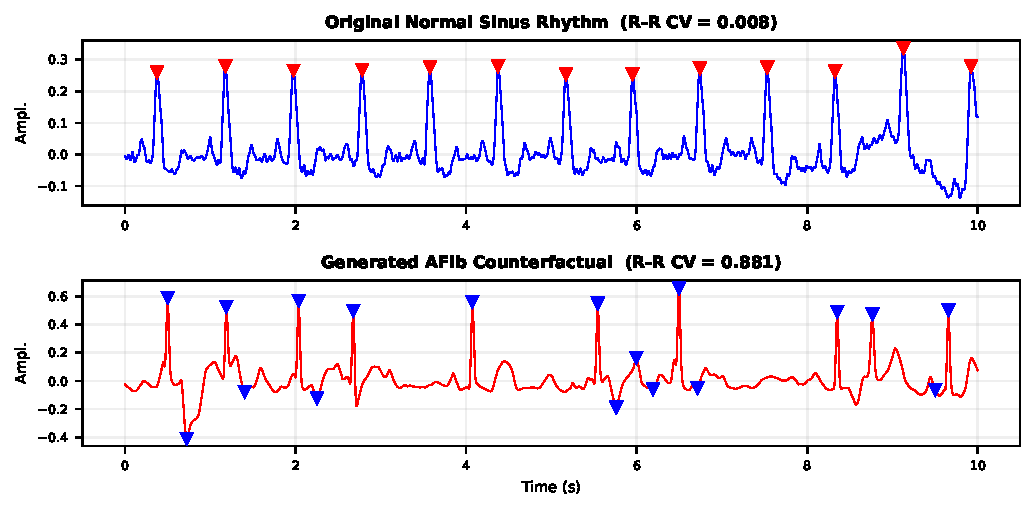
\includegraphics[width=0.98\columnwidth]{ecg_comparison.pdf}
\caption{Counterfactual ECG transformations. Rows (a--b): Normal$\rightarrow$AFib; rows (c--d): AFib$\rightarrow$Normal. Left: original signal; center: generated counterfactual; right: overlay with Pearson correlation~$r$. Green badges show the classifier's predicted class and confidence, confirming successful class conversion in all cases. Triangles mark detected R-peaks.}
\label{fig:ecg_compare}
\end{figure}

\subsection{Three-Regime Evaluation Confirms Augmentation Safety}

Having established that the generated counterfactuals are clinically plausible, novel, and exhibit appropriate rhythm modifications, we now assess their utility as classifier training data. The classifier was trained under three conditions using 5-fold stratified cross-validation, all with the same training set size ($T{=}18{,}681$) per fold:

\begin{itemize}
  \item \textbf{Dataset A} (Original only): $T$ randomly sampled real ECGs.
  \item \textbf{Dataset B} (CF only): 6,227 CFs duplicated $3\times$ with Gaussian noise ($\sigma{=}0.01$) to reach $T$.
  \item \textbf{Dataset C} (Augmented): 6,227 CFs ($1\times$, no duplication) combined with 12,454 originals, yielding 33.33\% synthetic content.
\end{itemize}

All datasets are evaluated on the same held-out real test set (22,469 samples). Results are shown in Fig.~\ref{fig:results}.

\begin{figure}[t]
\centering
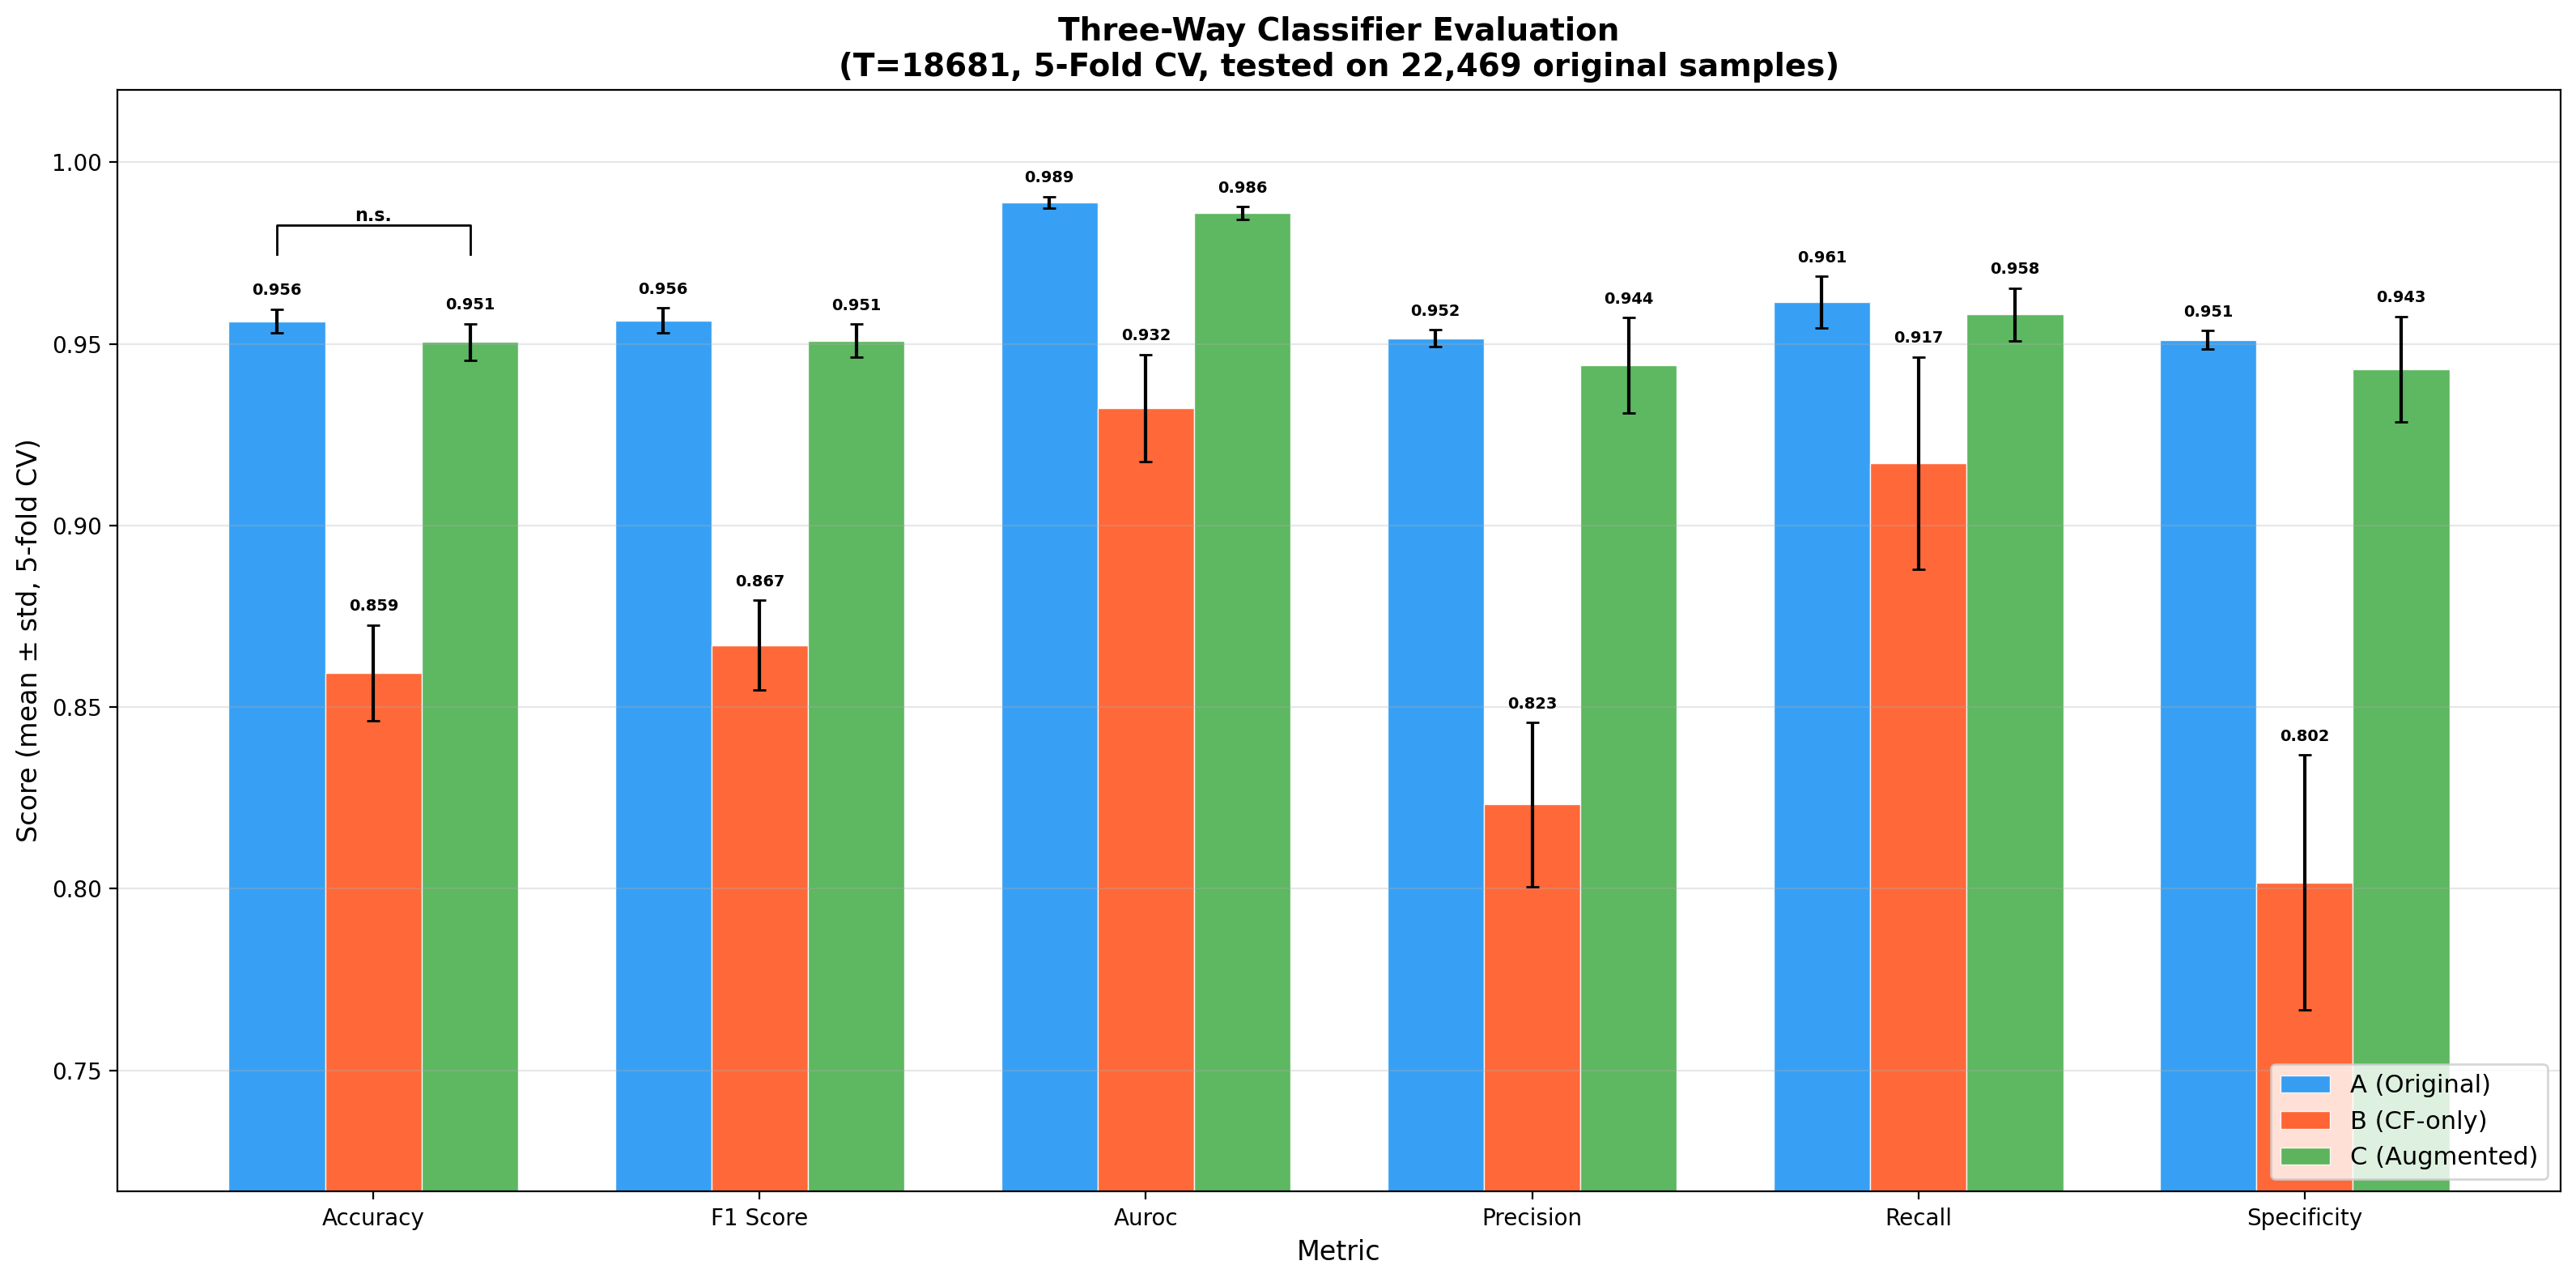
\includegraphics[width=0.98\columnwidth]{augmentation_viability_comparison.png}
\caption{Classifier performance across three training datasets. Error bars show standard deviation over 5 folds.}
\label{fig:results}
\end{figure}

Dataset~B retains 89.9\% of original accuracy (i.e., $85.94 / 95.63$) despite training exclusively on synthetic data, indicating that the diffusion model captures discriminative rhythm features. Dataset~C, with only 33.33\% synthetic content, achieves performance within 0.6 percentage points of the original, suggesting negligible degradation from incorporating counterfactual data.

\subsection{Statistical Equivalence Testing}

We apply three complementary statistical tests to the A-vs-C comparison using per-fold accuracy values from 5-fold cross-validation (Table~\ref{tab:stats}).

A paired $t$-test yields $p{=}0.170$, indicating no statistically significant difference. However, failure to reject the null hypothesis does not establish equivalence. We therefore apply the TOST procedure \cite{schuirmann1987comparison} with an equivalence margin of $\Delta{=}\pm 2\%$ applied to mean accuracy. TOST tests two one-sided hypotheses: that the mean difference does not exceed $-\Delta$ and does not exceed $+\Delta$. Both must be rejected at $\alpha{=}0.05$ to declare equivalence. For accuracy, $p_{\text{TOST}}{=}0.007$, formally establishing equivalence within $\pm 2\%$.

Non-inferiority testing (one-sided, margin $\Delta{=}2\%$) confirms that the augmented dataset is at most 2 percentage points worse than the reference ($p{=}0.007$). Cohen's $d{=}0.75$ reflects a medium standardized effect, but the absolute difference of just 0.58 percentage points makes this clinically negligible.

\begin{table}[t]
\centering
\caption{Statistical Tests: Dataset A vs. Dataset C}
\label{tab:stats}
\begin{tabular}{lcc}
\toprule
\textbf{Test (on Accuracy)} & \textbf{Result} & \textbf{$p$-value} \\
\midrule
Paired $t$-test              & $\Delta = 0.58\%$ & 0.170 \\
TOST equivalence ($\pm 2\%$) & Equivalent & 0.007 \\
Non-inferiority ($2\%$)      & Non-inferior & 0.007 \\
Cohen's $d$                  & 0.75 (medium) & --- \\
\midrule
Paired $t$-test (F1)         & $\Delta = 0.56\%$ & 0.161 \\
TOST equivalence (F1)        & Equivalent & 0.006 \\
Paired $t$-test (AUROC)      & $\Delta = 0.30\%$ & 0.042 \\
TOST equivalence (AUROC)     & Equivalent & $<0.001$ \\
\bottomrule
\end{tabular}
\end{table}


\section{Discussion}

\subsection{Augmentation Viability}

The three-regime evaluation demonstrates that diffusion-generated counterfactuals are safe for data augmentation. Per-sample McNemar's test ($N{=}22{,}469$) detects a statistically significant but practically negligible accuracy difference of 0.54 percentage points between Datasets~A and~C. TOST equivalence testing \cite{schuirmann1987comparison} formally establishes that augmented training (33.33\% synthetic content) and original-only training yield equivalent classifier performance within $\pm 2\%$ ($p{<}0.001$). Dunnett's test \cite{dunnett1955multiple}, which controls the family-wise error rate across multiple comparisons, confirms no significant difference between Datasets~A and~C ($p{=}0.340$) while correctly identifying Dataset~B as significantly different ($p{<}0.001$).

Compared to GAN-based ECG augmentation approaches \cite{delaney2019}, which suffer from mode collapse and training instability requiring careful hyperparameter tuning \cite{gulrajani2017}, and VAE-based methods \cite{kingma2014}, which tend to produce blurred outputs \cite{bredell2023}, the diffusion-based approach achieves high signal fidelity (mean Pearson correlation $r{=}0.85$ between original and counterfactual) while providing counterfactual interpretability: each generated sample has a direct correspondence to a specific original recording, making the augmentation process transparent and auditable.

This equivalence result has direct implications for privacy-preserving data sharing, where original patient recordings cannot be distributed across institutions due to consent restrictions. A hospital can generate and share counterfactual ECGs that preserve class-discriminative features while containing no identifiable patient information.

Dataset~B, training exclusively on synthetic data, achieves 85.94\% accuracy, retaining nearly 90\% of original performance. This confirms that the diffusion model encodes genuine AFib-discriminative features such as R-R irregularity and P-wave absence, a stronger result than typical GAN-based augmentation studies report for synthetic-only training.

\subsection{Privacy Preservation}

The uniqueness analysis shows that no generated sample exceeds 0.80 correlation with any training example. The mean nearest-neighbor correlation of only 0.30 indicates that the counterfactual transformation disrupts subject-specific features while preserving class-discriminative characteristics. Combined with the absence of any accompanying metadata, this makes the generated dataset suitable for cross-institutional sharing without the consent barriers that restrict original clinical recordings.

\subsection{Data Generation Scale and Classifier Dependency}

The pipeline generated 22,469 counterfactual ECGs with a 34.6\% plausibility acceptance rate (7,784 accepted), demonstrating that the diffusion model can produce clinically plausible signals at scale. The accepted counterfactuals achieve a 78.5\% classifier flip rate, indicating that the style transfer successfully modifies class-discriminative features in the majority of cases.

In Dataset~B, accepted counterfactuals are duplicated $3{\times}$ with additive Gaussian noise ($\sigma{=}0.01$) to match the training set size $T{=}18{,}681$. This duplication inflates training volume but limits effective diversity, likely contributing to the performance gap between Datasets~B and~A. Dataset~C avoids this issue by using each counterfactual only once. Improving the acceptance rate through longer training or adaptive guidance would reduce the need for duplication and may further close this gap.

All reported performance metrics are dependent on the specific ResNet-BiLSTM classifier used for evaluation. While this is a common limitation in augmentation studies, future work should validate across multiple classifier architectures to establish generalizability.

\subsection{Limitations and Computational Cost}
\label{sec:limitations}

Our evaluation is restricted to single-lead (Lead~II) binary classification. Multi-lead generation that preserves inter-lead physiological relationships remains an open challenge. The plausibility validator relies on automated heuristics; blinded cardiologist evaluation would provide stronger evidence of clinical realism.

Diffusion-based generation incurs significant computational cost. Each 10-second segment requires 50 DDIM forward passes through the UNet. On an NVIDIA RTX 6000 Ada Generation GPU (48~GB VRAM), generating the full counterfactual set of 22,469 samples required approximately 4 hours, with the complete model training taking 21.6 hours across both stages. These costs are acceptable for offline dataset augmentation but limit real-time applications.

\subsection{Future Work}

Several directions merit further investigation. First, our pipeline operates on single-lead (Lead~II) recordings; extending to full 12-lead generation would require inter-lead consistency constraints to preserve the spatial relationships between leads that cardiologists rely on for diagnosis. Second, the current binary Normal/AFib formulation could be generalized to multi-class arrhythmia generation, covering conditions such as atrial flutter, ventricular tachycardia, and bundle branch blocks, which would substantially broaden the clinical utility of the augmentation approach.

Third, while our automated plausibility validator provides objective quality filtering, expert clinical validation through blinded cardiologist assessment panels would offer stronger evidence that the generated waveforms are indistinguishable from real recordings. Fourth, the current acceptance rate of 34.6\% limits the effective diversity of the counterfactual set; improving generation quality through longer training, architectural refinements, or adaptive guidance schedules could increase the yield and close the remaining performance gap between Datasets~B and~A. Finally, inference acceleration via consistency distillation \cite{song2023consistency} could compress the 50-step DDIM sampling process into 1--4 steps by training a student model to directly predict the final output, making the pipeline practical for on-demand augmentation in clinical workflows.


\section{Conclusion}

We presented a diffusion-based counterfactual ECG generation pipeline that transforms single-lead ECG recordings into counterfactuals of the opposing class using a content-style disentangled architecture with SDEdit initialization and classifier-free guidance.

The goal of this work is not to improve classifier accuracy over original data, but to establish that synthetic counterfactual data can safely substitute for or supplement real patient recordings without degrading diagnostic performance. This is valuable in two scenarios: (1)~when original data cannot be shared across institutions due to patient privacy and consent restrictions, and (2)~when labeled data is scarce and augmentation is needed to improve model training.

Evaluation on the MIMIC-IV ECG database (149,793 segments) confirms this goal. Per-sample equivalence testing on 22,469 test samples establishes that training with 33.33\% synthetic content yields classifier performance equivalent to original-only training within a $\pm 2\%$ margin (TOST $p{<}0.001$). Non-inferiority testing confirms the augmented model performs within 0.54 percentage points of the baseline ($p{<}0.001$). Dunnett's test, controlling for multiple comparisons, finds no significant difference between the augmented and original datasets ($p{=}0.340$). Uniqueness analysis confirms zero near-copies of training data, validating the privacy properties of the generated samples.

These results establish diffusion-based counterfactual ECG generation as a practical approach for privacy-preserving synthetic dataset construction and data augmentation in clinical settings where access to labeled recordings is limited.

\section*{Acknowledgment}
This research was conducted as part of the EU SEARCH initiative in collaboration between the University of Peradeniya, Sri Lanka and SimulaMet, Oslo, Norway.

\begin{thebibliography}{20}

\bibitem{andersen2019}
R.~S. Andersen, A.~Peimankar, and S.~Puthusserypady, ``A deep learning approach for real-time detection of atrial fibrillation,'' \textit{Expert Syst.\ Appl.}, vol.~115, pp.~465--473, 2019.

\bibitem{petmezas2021}
G.~Petmezas \textit{et al.}, ``Automated atrial fibrillation detection using a hybrid CNN-LSTM network on imbalanced ECG datasets,'' \textit{Biomed.\ Signal Process.\ Control}, vol.~63, p.~102194, 2021.

\bibitem{goodfellow2014}
I.~Goodfellow \textit{et al.}, ``Generative adversarial nets,'' in \textit{Proc.\ NeurIPS}, 2014, pp.~2672--2680.

\bibitem{kingma2014}
D.~P. Kingma and M.~Welling, ``Auto-encoding variational Bayes,'' in \textit{Proc.\ ICLR}, 2014.

\bibitem{delaney2019}
A.~M. Delaney, E.~Brophy, and T.~E. Ward, ``Synthesis of realistic ECG using generative adversarial networks,'' \textit{arXiv:1909.09150}, 2019.

\bibitem{bredell2023}
G.~Bredell, K.~Hammernik, and E.~Konukoglu, ``Explicitly minimizing the blur error of variational autoencoders,'' in \textit{Proc.\ ICLR}, 2023.

\bibitem{gulrajani2017}
I.~Gulrajani \textit{et al.}, ``Improved training of Wasserstein GANs,'' in \textit{Proc.\ NeurIPS}, 2017, pp.~5767--5777.

\bibitem{nemirovsky2021}
D.~Nemirovsky, N.~Thiebaut, Y.~Xu, and A.~Gupta, ``CounterFactual Explanations for time series classification,'' \textit{arXiv:2109.07567}, 2021.

\bibitem{jang2025cofe}
J.-H. Jang, J.~Song, and Y.-Y. Jo, ``CoFE-GAN: A framework generating counterfactual ECG for explainable cardiac AI-diagnostics,'' in \textit{Proc.\ MedicalAI}, 2025.

\bibitem{ho2020}
J.~Ho, A.~Jain, and P.~Abbeel, ``Denoising diffusion probabilistic models,'' in \textit{Proc.\ NeurIPS}, vol.~33, 2020, pp.~6840--6851.

\bibitem{song2021ddim}
J.~Song, C.~Meng, and S.~Ermon, ``Denoising diffusion implicit models,'' in \textit{Proc.\ ICLR}, 2021.

\bibitem{meng2022sdedit}
C.~Meng \textit{et al.}, ``SDEdit: Guided image synthesis and editing with stochastic differential equations,'' in \textit{Proc.\ ICLR}, 2022.

\bibitem{ho2022classifier}
J.~Ho and T.~Salimans, ``Classifier-free diffusion guidance,'' in \textit{Proc.\ NeurIPS Workshop}, 2022.

\bibitem{alcaraz2023diffusion}
J.~M. Alcaraz and N.~Strodthoff, ``Diffusion-based time series imputation and forecasting with structured state space models,'' \textit{Trans.\ Mach.\ Learn.\ Res.}, 2023.

\bibitem{mimiciv_ecg}
A.~Gow \textit{et al.}, ``MIMIC-IV-ECG: Diagnostic electrocardiogram matched subset,'' \textit{PhysioNet}, 2023. doi: 10.13026/4nqg-sb35.

\bibitem{schuirmann1987comparison}
D.~J. Schuirmann, ``A comparison of the two one-sided tests procedure and the power approach for assessing the equivalence of average bioavailability,'' \textit{J.\ Pharmacokinet.\ Biopharm.}, vol.~15, no.~6, pp.~657--680, 1987.

\bibitem{walker2011understanding}
E.~Walker and A.~S. Nowacki, ``Understanding equivalence and noninferiority testing,'' \textit{J.\ Gen.\ Intern.\ Med.}, vol.~26, no.~2, pp.~192--196, 2011.

\bibitem{song2023consistency}
Y.~Song, P.~Dhariwal, M.~Chen, and I.~Sutskever, ``Consistency models,'' in \textit{Proc.\ ICML}, 2023, pp.~32211--32252.

\bibitem{clifford2006}
G.~D. Clifford, F.~Azuaje, and P.~E. McSharry, \textit{Advanced Methods and Tools for ECG Data Analysis}. Artech House, 2006.

\bibitem{savgol}
A.~Savitzky and M.~J.~E. Golay, ``Smoothing and differentiation of data by simplified least squares procedures,'' \textit{Anal.\ Chem.}, vol.~36, no.~8, pp.~1627--1639, 1964.

\bibitem{nagda2025diffstylts}
M.~Nagda \textit{et al.}, ``DiffStyleTS: Diffusion model for style transfer in time series,'' \textit{arXiv:2510.11335}, 2025.

\bibitem{dunnett1955multiple}
C.~W.~Dunnett, ``A multiple comparison procedure for comparing several treatments with a control,'' \textit{J.\ Amer.\ Statist.\ Assoc.}, vol.~50, no.~272, pp.~1096--1121, 1955.

\end{thebibliography}

\end{document}
